\documentclass[10pt]{article}
\usepackage[T1]{fontenc}

% Document Details
\newcommand{\CLASS}{AMATH 563}
\newcommand{\assigmentnum}{Networks}

\usepackage[margin = 1in, left=0.75in,right=0.75in]{geometry}
\usepackage{titling}
\setlength{\droptitle}{-6em}   % This is your set screw
\date{}
\renewcommand{\maketitle}{
	\clearpage
	\begingroup  
	\centering
	\LARGE \sffamily\textbf{\CLASS} \Large \assigmentnum\\[.8em]
	\large Tyler Chen\\[1em]
	\endgroup
	\thispagestyle{empty}
}
 % Title Styling


\usepackage{enumitem}

% Figures
\usepackage{subcaption}

% TikZ and Graphics
\usepackage{tikz, pgfplots}
\pgfplotsset{compat=1.12}
\usetikzlibrary{patterns,arrows}
\usepgfplotslibrary{fillbetween}

\usepackage{pdfpages}
\usepackage{adjustbox}

\usepackage{lscape}
\usepackage{titling}
\usepackage[]{hyperref}


% Header Styling
\usepackage{fancyhdr}
\pagestyle{fancy}
\lhead{\sffamily \CLASS}
\rhead{\sffamily Chen \textbf{\thepage}}
\cfoot{}

% Paragraph Styling
\setlength{\columnsep}{1cm}
\setlength{\parindent}{0pt}
\setlength{\parskip}{5pt}
\renewcommand{\baselinestretch}{1}

% TOC Styling
\usepackage{tocloft}
\iffalse
\renewcommand{\cftsecleader}{\cftdotfill{\cftdotsep}}

\renewcommand\cftchapafterpnum{\vskip6pt}
\renewcommand\cftsecafterpnum{\vskip10pt}
\renewcommand\cftsubsecafterpnum{\vskip6pt}

% Adjust sectional unit title fonts in ToC
\renewcommand{\cftchapfont}{\sffamily}
\renewcommand{\cftsecfont}{\bfseries\sffamily}
\renewcommand{\cftsecnumwidth}{2em}
\renewcommand{\cftsubsecfont}{\sffamily}
\renewcommand{\cfttoctitlefont}{\hfill\bfseries\sffamily\MakeUppercase}
\renewcommand{\cftaftertoctitle}{\hfill}

\renewcommand{\cftchappagefont}{\sffamily}
\renewcommand{\cftsecpagefont}{\bfseries\sffamily}
\renewcommand{\cftsubsecpagefont}{\sffamily}
\fi
 % General Styling
% Code Display Setup
\usepackage{listings,lstautogobble}
\usepackage{lipsum}
\usepackage{courier}
\usepackage{catchfilebetweentags}

\lstset{
	basicstyle=\small\ttfamily,
	breaklines=true, 
	frame = single,
	rangeprefix=,
	rangesuffix=,
	includerangemarker=false,
	autogobble = true
}


\usepackage{algorithmicx}
\usepackage{algpseudocode}

\newcommand{\To}{\textbf{to}~}
\newcommand{\DownTo}{\textbf{downto}~}
\renewcommand{\algorithmicdo}{\hspace{-.2em}\textbf{:}}
 % Code Display Setup
% AMS MATH Styling
\usepackage{amsmath, amssymb}
\newcommand{\qed}{\hfill\(\square\)}

%\newtheorem*{lemma}{Lemma} 
%\newtheorem*{theorem}{Theorem}
%\newtheorem*{definition}{Definition}
%\newtheorem*{prop}{Proposition}
%\renewenvironment{proof}{{\bfseries Proof.}}{}


% mathcal
\newcommand{\cA}{\ensuremath{\mathcal{A}}}
\newcommand{\cB}{\ensuremath{\mathcal{B}}}
\newcommand{\cC}{\ensuremath{\mathcal{C}}}
\newcommand{\cD}{\ensuremath{\mathcal{D}}}
\newcommand{\cE}{\ensuremath{\mathcal{E}}}
\newcommand{\cF}{\ensuremath{\mathcal{F}}}
\newcommand{\cG}{\ensuremath{\mathcal{G}}}
\newcommand{\cH}{\ensuremath{\mathcal{H}}}
\newcommand{\cI}{\ensuremath{\mathcal{I}}}
\newcommand{\cJ}{\ensuremath{\mathcal{J}}}
\newcommand{\cK}{\ensuremath{\mathcal{K}}}
\newcommand{\cL}{\ensuremath{\mathcal{L}}}
\newcommand{\cM}{\ensuremath{\mathcal{M}}}
\newcommand{\cN}{\ensuremath{\mathcal{N}}}
\newcommand{\cO}{\ensuremath{\mathcal{O}}}
\newcommand{\cP}{\ensuremath{\mathcal{P}}}
\newcommand{\cQ}{\ensuremath{\mathcal{Q}}}
\newcommand{\cR}{\ensuremath{\mathcal{R}}}
\newcommand{\cS}{\ensuremath{\mathcal{S}}}
\newcommand{\cT}{\ensuremath{\mathcal{T}}}
\newcommand{\cU}{\ensuremath{\mathcal{U}}}
\newcommand{\cV}{\ensuremath{\mathcal{V}}}
\newcommand{\cW}{\ensuremath{\mathcal{W}}}
\newcommand{\cX}{\ensuremath{\mathcal{X}}}
\newcommand{\cY}{\ensuremath{\mathcal{Y}}}
\newcommand{\cZ}{\ensuremath{\mathcal{Z}}}

% mathbb
\usepackage{bbm}
\newcommand{\bOne}{\ensuremath{\mathbbm{1}}}

\newcommand{\bA}{\ensuremath{\mathbb{A}}}
\newcommand{\bB}{\ensuremath{\mathbb{B}}}
\newcommand{\bC}{\ensuremath{\mathbb{C}}}
\newcommand{\bD}{\ensuremath{\mathbb{D}}}
\newcommand{\bE}{\ensuremath{\mathbb{E}}}
\newcommand{\bF}{\ensuremath{\mathbb{F}}}
\newcommand{\bG}{\ensuremath{\mathbb{G}}}
\newcommand{\bH}{\ensuremath{\mathbb{H}}}
\newcommand{\bI}{\ensuremath{\mathbb{I}}}
\newcommand{\bJ}{\ensuremath{\mathbb{J}}}
\newcommand{\bK}{\ensuremath{\mathbb{K}}}
\newcommand{\bL}{\ensuremath{\mathbb{L}}}
\newcommand{\bM}{\ensuremath{\mathbb{M}}}
\newcommand{\bN}{\ensuremath{\mathbb{N}}}
\newcommand{\bO}{\ensuremath{\mathbb{O}}}
\newcommand{\bP}{\ensuremath{\mathbb{P}}}
\newcommand{\bQ}{\ensuremath{\mathbb{Q}}}
\newcommand{\bR}{\ensuremath{\mathbb{R}}}
\newcommand{\bS}{\ensuremath{\mathbb{S}}}
\newcommand{\bT}{\ensuremath{\mathbb{T}}}
\newcommand{\bU}{\ensuremath{\mathbb{U}}}
\newcommand{\bV}{\ensuremath{\mathbb{V}}}
\newcommand{\bW}{\ensuremath{\mathbb{W}}}
\newcommand{\bX}{\ensuremath{\mathbb{X}}}
\newcommand{\bY}{\ensuremath{\mathbb{Y}}}
\newcommand{\bZ}{\ensuremath{\mathbb{Z}}}

% alternative mathbb
\newcommand{\NN}{\ensuremath{\mathbb{N}}}
\newcommand{\RR}{\ensuremath{\mathbb{R}}}
\newcommand{\CC}{\ensuremath{\mathbb{C}}}
\newcommand{\ZZ}{\ensuremath{\mathbb{Z}}}
\newcommand{\EE}{\ensuremath{\mathbb{E}}}
\newcommand{\PP}{\ensuremath{\mathbb{P}}}
\newcommand{\VV}{\ensuremath{\mathbb{V}}}
\newcommand{\cov}{\ensuremath{\text{Co}\VV}}
% Math Commands

\newcommand{\st}{~\big|~}
\newcommand{\stt}{\text{ st. }}
\newcommand{\ift}{\text{ if }}
\newcommand{\thent}{\text{ then }}
\newcommand{\owt}{\text{ otherwise }}

\newcommand{\norm}[1]{\left\lVert#1\right\rVert}
\newcommand{\snorm}[1]{\lVert#1\rVert}
\newcommand{\ip}[1]{\ensuremath{\left\langle #1 \right\rangle}}
\newcommand{\pp}[3][]{\frac{\partial^{#1}#2}{\partial #3^{#1}}}
\newcommand{\dd}[3][]{\frac{\d^{#1}#2}{\d #3^{#1}}}
\renewcommand{\d}{\ensuremath{\mathrm{d}}}

\newcommand{\indep}{\rotatebox[origin=c]{90}{$\models$}}




 % Math shortcuts

\usepackage{dblfloatfix}    % To enable figures at the bottom of page

% Problem
\newenvironment{problem}[1]{\vspace{2em}{\large\sffamily\textbf{#1}}\itshape\par}{}

\usepackage{nameref}
\newcommand{\vln}{\rotatebox{90}{--}}

\begin{document}

\twocolumn[{%
\begin{@twocolumnfalse}
\maketitle
\vspace{2em}
\begin{abstract}
We take connectivity graphs of neurons in the c. elegans worm and analyze the connectivity. This is done first using a graph theoretic approach, and then an approach based on the Kuramoto Oscillator.
\end{abstract}

\vspace{4em}
%\tableofcontents
%\vspace{3em}
\pagebreak\end{@twocolumnfalse}
}]

\section{Introduction and Overview}
Networks arise naturally in a variety of applications. Being able to understand the behavior of large networks is of clear interest. In this report we compute degree and flow distributions of the adjacency matrix for the chemical synaptic network (directed) and adjacency matrix for the gap junction network (undirected). We then compute the diameter of the communication classes of each of these networks as well as the combination. We also put these graphs into the Kuramoto oscillator model and observe how the coupled the resulting systems are.

\section{Theoretical Background}

\subsection{Graphs}
We provided a basic introduction to the definitions used in graph theory \cite{graph_notes}.

Given some vertex set \( V \), an undirected graph is the tuple \( G = (V,E) \), where the edge set \( E \) contains elements of the form \( e=\{u,v\} \) where \( u,v\in G \).

The degree of a node \( v\in V \) is the number of edges in \( E \) containing \( v \). The flow of a node \( v \) is the sum of the weights of the edges containing \( v \).

A subgraph \( G' \) of \( G \) is a graph formed by taking a subsets \( V' \subseteq V \) and \( E'\subseteq E \) such that every endpoint of \( E' \) is in \( V' \).

The subgraph of \( G \) induced by \( V' \) is the graph \( G' = (V',E') \) where \( E' = \{ \{u,v\} : u,v\in V' \} \).

A \( u \)-\( v \) path is a list of the form \( p = (u=v_0,v_1,v_2,\ldots, v_k=v) \) such that \( \{v_j,v_{j+1}\}\in E \) for \( j=0,\ldots, k-1 \). If such a path exists we say that \( v \) is reachable from \( u \).

Clearly this gives gives rise to the notion of reachibility. That is, which vertices can be reached from which vertices. This forms an equivalence relation, where the equivalence classes are called the connected components of \( G \).

We say the graph \( G \) is connected if there exists a \( u \)-\( v \) path between every pair of vertices \( u,v\in V \). Equivalently, that there is only one connected component.

A weighting on the graph \( G \) is a function \( w:E\to \bR \). The weight of a \( u-v \) path is the sum of the weights of the edges in this path.

A minimum length  \( u \)-\( v \) path is a \( u \)-\( v \) path such that any other \( u \)-\( v \) path is longer (has more edges). A minimum weight \( u \)-\( v \) path is a \( u \)-\( v \) path such that any other \( u \)-\( v \) path has a larger weight.

The diameter of \( G \) is the length of the longest minimum length path between all pairs of vertices in \( V \). If the graph is not connected the diameter is taken to be infinite.

Up to this point everything we have done has been relating to undirected graphs. Given some vertex set \( V \), an undirected graph is the tuple \( G = (V,E) \), where the edge set \( E \) contains elements of the form \( e=(u,v) \) where \( u,v\in G \). We now note that \( (u,v)\in E \) does not imply \( (v,u)\in E \).

Instead of the degree of a node \( v \), we have the in-degree and the out-degree. Respectively these are the number of edges ending and starting at \( v \). Similarly we have in-flow and out-flow.

A subgraph of a directed graph is defined in the same way as for an undirected graph. Similarly, a \( u \)-\( v \) path is defined in the same way.

\begin{figure*}[b]\centering
\begin{subfigure}{.3\textwidth}\centering
    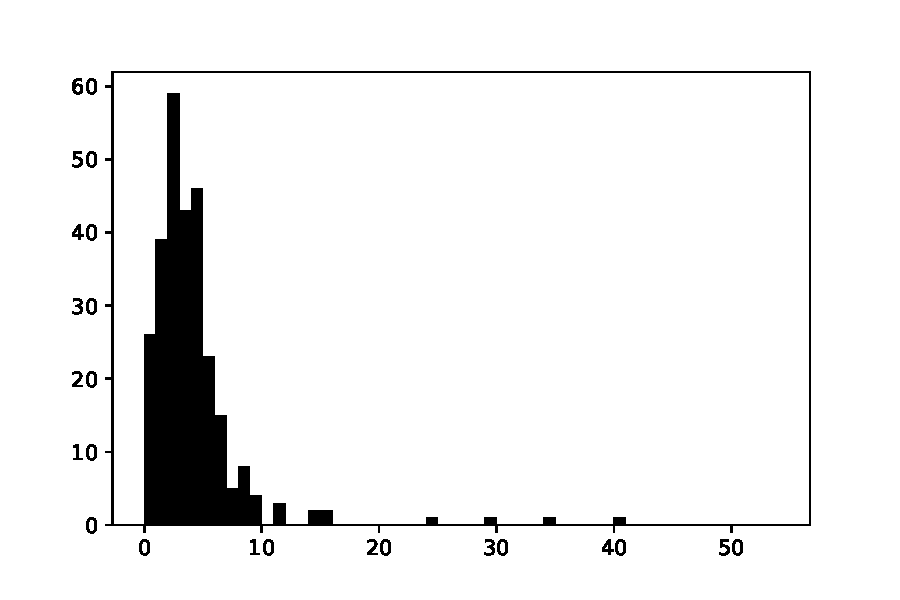
\includegraphics[width=\textwidth]{img/L_deg.pdf}
    \caption{\(L\) degree distribution}
\end{subfigure}\hfill
\begin{subfigure}{.3\textwidth}\centering
    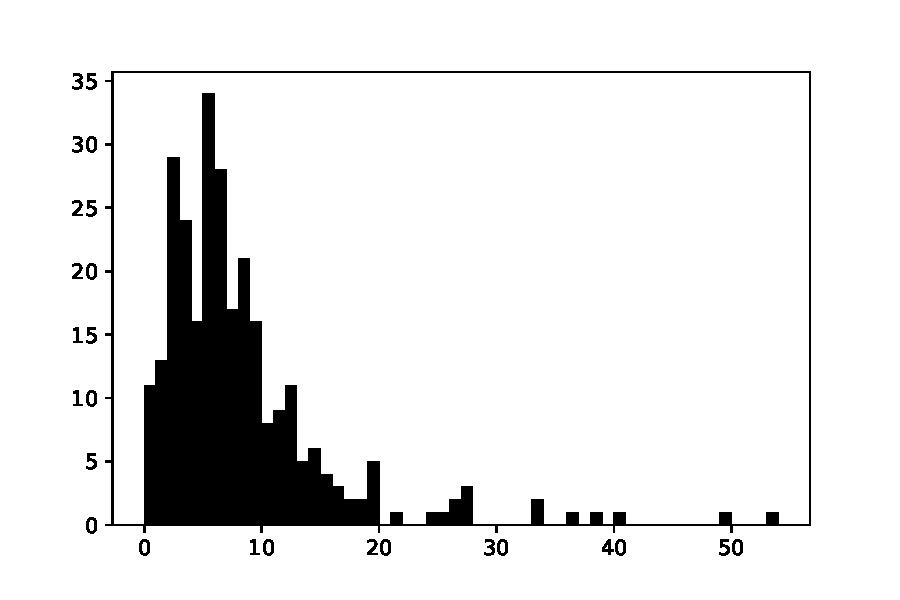
\includegraphics[width=\textwidth]{img/Ac_deg_in.pdf}
    \caption{\(A_c\) in-degree distribution}
\end{subfigure}\hfill
\begin{subfigure}{.3\textwidth}\centering
    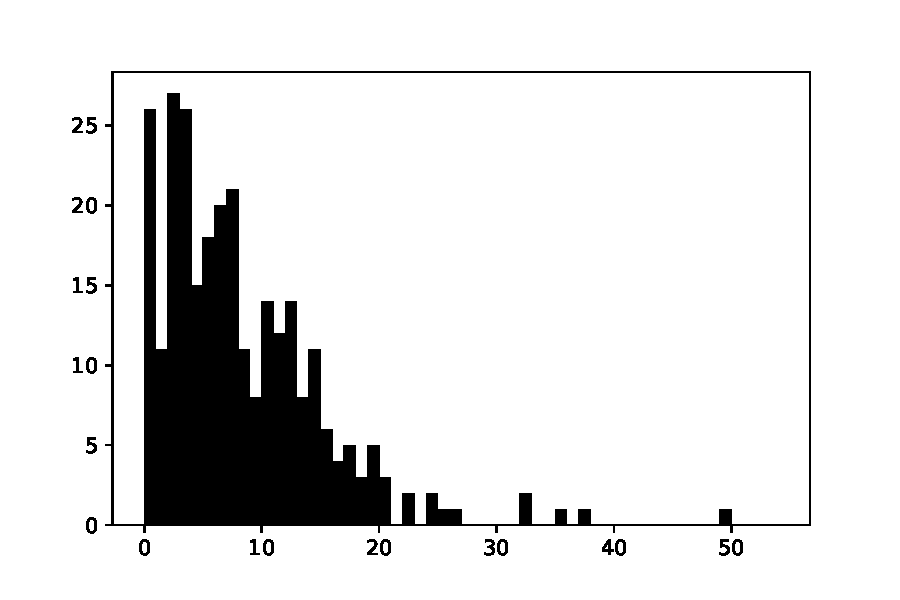
\includegraphics[width=\textwidth]{img/Ac_deg_out.pdf}
    \caption{\(A_c\) out-degree distribution}
\end{subfigure}
\caption{Degree Distributions (horizontal: degree, vertical: count)}
\label{degrees}
\end{figure*}

However, reachability no longer forms an equivalence relation. Instead of connected components we can define communication classes to be the maximal subgraphs for which there is a path between any pair of nodes in the subgraph.

We say a directed graph is strongly connected if every vertex is reachable from every other vertex. Equivalently, that there is a single communication class. We say a directed graph is weakly connected if, treating all edges as undirected, the graph is connected.

Weighting on a directed graph is defined in the same way as for an undirected graph.

The diameter of directed graph is the longest minimum length path between all pairs of vertices in \( V \). If a vertex is unreachable from any other vertex the diameter is take to be infinite.

\subsection{Kuramoto Oscillator}
The Kuramoto model describes the behavior of a large set of coupled oscillators \cite{lecture_notes}.

Given \( N \) oscillators, their phases \( \theta_i \) are given by the differential equation,
\begin{align}
    \dd{\theta_i}{t} = \omega_i + \dfrac{K}{N} \sum_{j=1}^{N} A_{ij}\sin(\theta_i-\theta_j) \label{kuramoto}
\end{align}
where each oscillator as natural frequency \( w_i \) and \( K \) and \( A \) gives the coupling strengths.

In order to measure ``how coupled'' a system is. We define the order parameters \( r \) and \( \psi \) by,
\begin{align}
    re^{i\psi} = \dfrac{1}{N} \sum_{j=1}^{N} e^{i\theta_j} \label{coherence}
\end{align}
where \( r \) is the phase coherence and \( \psi \) is the mean phase.

Note that \( e^{i\theta_j} \) will be somewhere on the unit circle, with argument given by the phase (value of \( \theta_j \) modulo \( 2\pi \)). If all the oscillators have a similar phase the mean of \( e^{i\theta_j} \) will have a modulus close to one and argument close to the shared phase. Conversely, if the oscillators have completely different phases, the means of \( e^{i\theta_j} \) will be somewhere near the origin.

Therefore, the value of \( r \) will give a measure of how similar the phases are at a given time. Taking the average value of \( r \) over some period of time after the oscillator has relaxed to a ``steady state'' will give a measure of how coupled the system is. Since \( |e^{i\theta_j}| = 1 \), \( r = 1 \) if all the phases are exactly the same. Otherwise, \( r \) will be smaller.

We can vary \( K \) and observe how \( r \) changes. Doing this for various \( A \) allows for the connectivity of various graphs to be compared. We know that as \( K \) increases the system will become increasingly coupled, however how quickly this happens will depend on how connected the oscillators are (sparsity of \( A \)) and other properties of the graph \( A \).

\begin{figure*}[t]\centering
\begin{subfigure}{.3\textwidth}\centering
    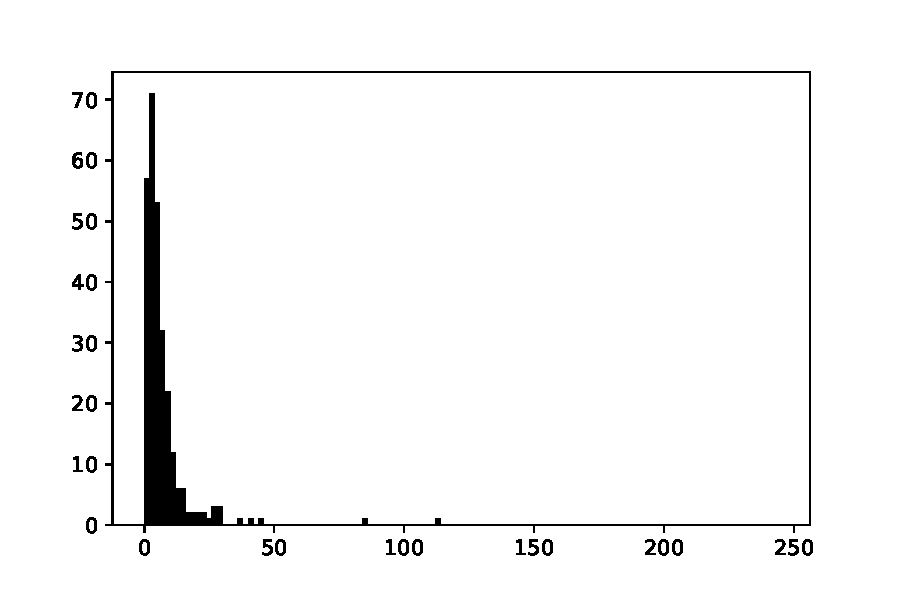
\includegraphics[width=\textwidth]{img/L_flow.pdf}
    \caption{\(L\) flow distribution}
\end{subfigure}\hfill
\begin{subfigure}{.3\textwidth}\centering
    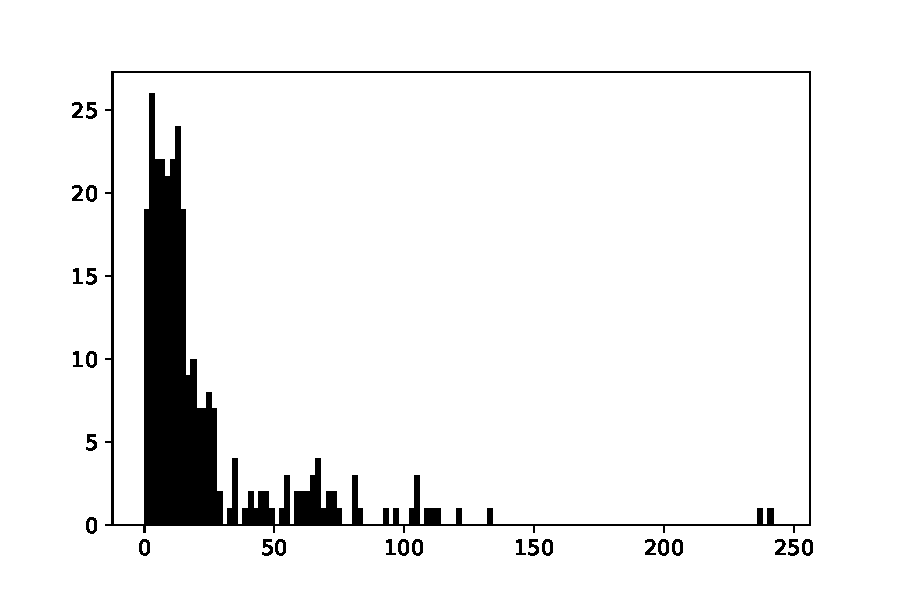
\includegraphics[width=\textwidth]{img/Ac_flow_in.pdf}
    \caption{\(A_c\) in-flow distribution}
\end{subfigure}\hfill
\begin{subfigure}{.3\textwidth}\centering
    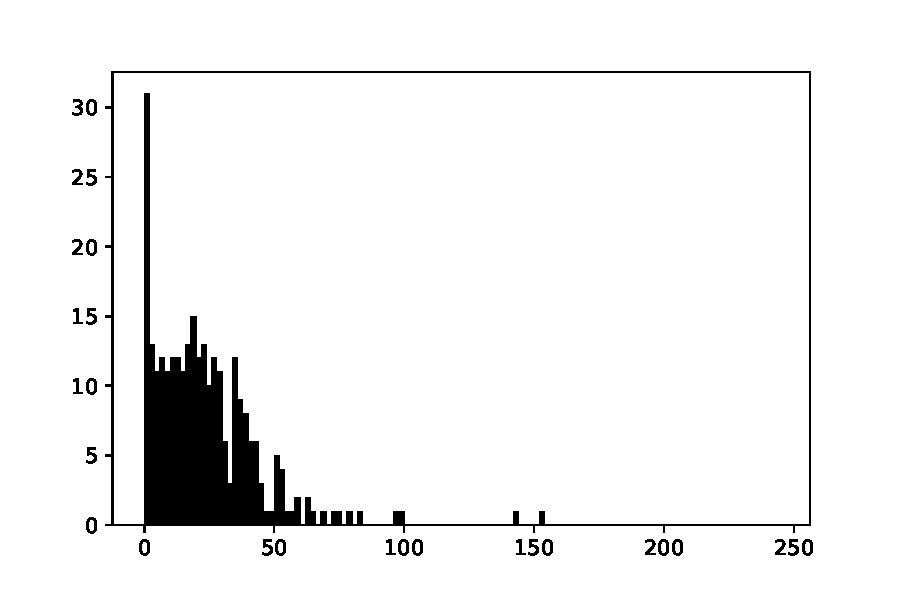
\includegraphics[width=\textwidth]{img/Ac_flow_out.pdf}
    \caption{\(A_c\) out-flow distribution}
\end{subfigure}
\caption{Flow Distributions (horizontal: flow, vertical: count)}
\label{flows}
\end{figure*}

\begin{figure*}[b]\centering
\foreach \k in {0,10,50}{
\begin{subfigure}{.3\textwidth}\centering
    \includegraphics[width=\textwidth]{img/phase/C_\k.pdf}
    \caption{\( K = \k \)}
 \end{subfigure}
}
\caption{Coupling strength \( K \) (horizontal) vs. phases (vertical) for couplings given by \( C \)}
\label{phase}
\end{figure*}


\section{Algorithm Implementation and Development}
All functions we use are taken from Scipy or core Python. In particular, we implement the Kuramoto Oscillator using scipy's {\tt solve\_ivp} and graph results are done using Scipy's {\tt sparse.csgraph} module. While our graphs are not sparse this was the most easily accessible module with functions to compute the number of connected components of a graph as well as the distance between any two nodes.

\subsection{Representing Graphs}
Graphs are represented using weighted adjacency matrices. To compute quantities such as diameter we convert the weighted adjacency graphs to unweighted ones, where the \( i,j \) entry is {\tt True} if there is an edge from \( i \) to \( j \) and {\tt False} otherwise.

To convert an directed unweighted adjacency graph \( G \) to an undirected one we simply take \( G \oplus G^T \) where \( \oplus \) indicates boolean {\tt or} applied componentwise to \( G \) and \( G^T \).

\subsection{Degree Distribution}
The in-degree and out-degree of a vertex can be found by counting the number of nonzero entries in the corresponding column or row. In the case of an undirected graph these numbers are the same. Given a graph Laplacian we can also just take the diagonal entry.

\subsection{Communication Classes}
We can easily find which vertices belong to which communication class using {\tt connected\_components} and the appropriate keywords.

\subsection{Diameter}
We compute the diameter of a communication class by applying Dijkstra to each node pair and taking the maximum.


\section{Computational Results}

We are given data about the connectivity of neurons in the c. elegans worm. In particular, \( A_c \) is the adjacency matrix for the chemical synaptic network (directed) and \( L \) is the Laplacian matrix for the gap junction network (undirected). We immediately replace \( L \) with the adjacency matrix and from now on use \( L \) to denote the adjacency matrix rather than the graph Laplacian. The nodes of the two graphs are identical.

Note that since no background on what the weights of the graphs mean it is not necessarily meaningful to compare the graphs in this way. In fact, this was a major concern through out this process. Since we do not know whether a higher weight should at all correspond to a higher coupling, it is not clear that using the connections as the coupling makes any sense.

\begin{figure*}[t]\centering
\begin{subfigure}{.48\textwidth}\centering
    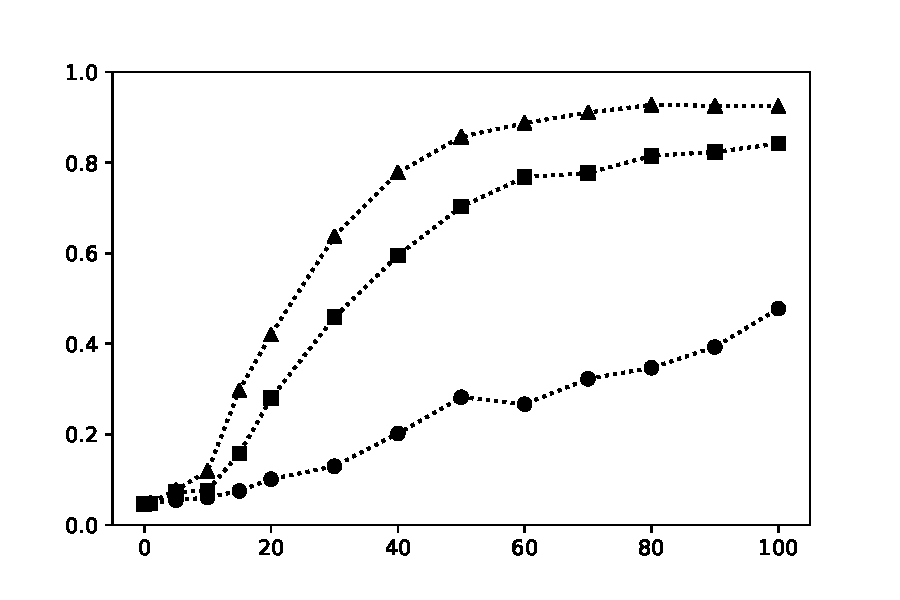
\includegraphics[width=\textwidth]{img/couple_strength.pdf}
    \caption{Unweighted adjacency graph}
    \label{couplinguw}
\end{subfigure}\hfill
\begin{subfigure}{.48\textwidth}\centering
    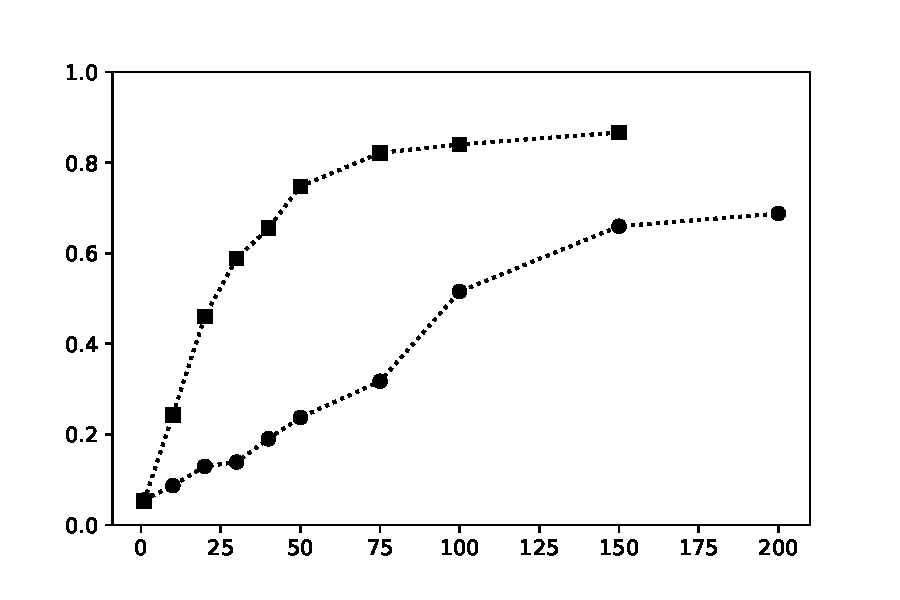
\includegraphics[width=\textwidth]{img/couple_strength_g.pdf}
    \caption{Weighted adjacency graph}
    \label{couplingw}
\end{subfigure}
\caption{Coupling strength \( K \) (horizontal) vs. phase coherence \( r \) (vertical). circles: \( L \), squares: \( A_c \), triangles: \( C \).}
\label{coupling}
\end{figure*}

\subsection{Graph Properties}
Figure~\ref{degrees} shows the degree distributions of \( L \) and \( A_c \). Similarly, Figure~\ref{flows} shows the flow distributions of \( L \) and \( A_c \). We immediately note that since both graphs have some nodes with degree zero that they are not connecte and so the diameters are infinite.

We next compute the connected components of \( L \) and the communication classes of \( A_c \).

The undirected graph \( L \) has 29 connected components. The non-trivial components have 248, 3, and 2 nodes and have diameters 12, 2, and 1. The rest of the components are isolated nodes.

We note that \( A_c \) is weakly connected. The directed graph \( A_c \) has 42 communication classes. There  non-trivial communication classes have 237 and 2 nodes and  have diameters 10 and 1.

The diameter of \( A_c \) where all edges are treated as undirected is 6.

Since both \( L \) and \( A_c \) share the same nodes we combine them into a graph denoted \( C \) by combining the unweighted adjacency matrices component using a logical {\tt or}. This means every edge of \( L \) or \( A_c \) is contained in \( C \).

The resulting directed graph is weakly connected and has 6 communication classes. The one non-trivial communication class has 274 nodes and diameter 7.

The diameter of \( C \) treated as an undirected graph is 5.

We note that combining \( L \) and \( A_c \) significantly reduces the number of communication classes as well as the diameter of the largest communication class despite the fact taht the  largest communication class of \( C \) has more node than those of \( A_c \) and \( L \). This is not necessarily surprising as we have combined two graphs.



\subsection{Kuramoto Oscillator}
We now solve the Kuramoto Oscillator system. In particular, we pick natural frequencies randomly from a uniform distribution on \( [1/2,3/2] \) and random initial phases uniformly on \( [0,2\pi] \).

We iterate over various values of \( K \) and compute \( r \) for the unweighted and weighted adjacency graphs of \( L \), \( A_c \), and the combination graph \( C \).

Figure~\ref{phase} shows the phases of the oscillators over time at various values of \( K \). Each oscillator has its path drawn with some opacity. Therefore, if most of the oscillators end up locked together the group phase should be clear. As expected, as \( K \) increases the phase locking becomes stronger.


Figure~\ref{coupling} shows the phase coherence as a function of the coupling strength for the unweighted adjacency graphs of \( L \), \( A_c \), and \( C \). As expected, as \( K \) increases the phase coherence increases for all graphs. Moreover, the more connected a graph is the lower the value of \( K \) has to be to reach a fixed coherence value.

While there is a slight difference between Figures~\ref{couplinguw} and \ref{couplingw}, the general behavior is the same. The most notable differences are near the origin, where the unweighted adjacency graphs have a much slower increase in coupling. 
We would have liked to increase \( K \) even further, however some of the data points took over an hour to generate. Given more time it would be trivial extend these plots.

Since it is not clear what the objective of this model is we do not continue this further. However, we note that no matter how large the coupling strength, disconnected components will not couple together. This means that there could be multiple coupled groups traveling independently from one another. That said, we do not need the oscillator model to determine that the graphs have connected components.


\section{Summary and Conclusions}
We compute degree and flow distributions of the adjacency matrix for the chemical synaptic network (directed) and adjacency matrix for the gap junction network (undirected). We then compute the diameter of the communication classes of each of these networks as well as the combination. Since we have no physical understanding of what our data means, we look which nodes are connected rather than the strength of these connections.

We put these graphs into the Kuramoto oscillator model and are able to observe how the phase coherence increases as the coupling strength increases. In particular we notice that the more connected the graphs are the quicker they become coupled. For instance, since \( C \) is a supergraph of \( L \) and \( A_c \), it is not surprising that the Kuramoto oscillator with coupling described by \( C \) becomes coherent at a lower value of \( K \) than the oscillators corresponding to either \( K \) or \( A_c \).

Overall we found it very unclear what the purpose of computing any of these quantities was. Since only very limited information was given about what \( L \) and \( A_c \) represent it is not clear that we can combine the data in any meaningful way. More specifically, if we knew that the weights represented the strength of connection, or time for a signal to travel the connection, etc, then a distance metric could be defined for the graphs and we could discuss physical quantities such as how long it would take a signal to travel between two nodes, etc. However, without knowing this we are reduced to observing topological properties of the graphs.


\bibliographystyle{plain}
\bibliography{hw4}

\onecolumn
\section{Appendix A}
\label{AppendixA}
All functions are included in the code in Appendix B as they are specific to the task performed in each of the files.

%\pagebreak
\section{Appendix B}
\lstinputlisting[]{hw4.py}


\end{document}
